% AI-Generated LaTeX Code Snippets
% SUZA Workshop - Day 3: AI Integration
% Examples of LaTeX code generated with AI assistance

\documentclass[12pt, a4paper]{article}

\usepackage[utf8]{inputenc}
\usepackage[margin=1in]{geometry}
\usepackage{graphicx}
\usepackage{amsmath, amssymb}
\usepackage{booktabs}
\usepackage{algorithm2e}
\usepackage{listings}
\usepackage{xcolor}
\usepackage{tikz}
\usetikzlibrary{shapes, arrows, positioning}
\usepackage{hyperref}

% Code listing settings
\lstset{
    backgroundcolor=\color{gray!10},
    basicstyle=\ttfamily\small,
    keywordstyle=\color{blue},
    commentstyle=\color{gray},
    stringstyle=\color{red},
    frame=single,
    breaklines=true,
    numbers=left
}

\title{AI-Generated LaTeX Code Examples}
\author{Generated with AI Assistance\\
        SUZA Scientific Writing Workshop}
\date{\today}

%==============================================================================
\begin{document}

\maketitle

\begin{abstract}
This document showcases various LaTeX code snippets that were generated using AI tools like ChatGPT and Claude. Each example demonstrates how AI can assist with creating tables, equations, algorithms, diagrams, and other LaTeX elements. All code has been verified to compile correctly and represents common academic writing needs.
\end{abstract}

\tableofcontents
\newpage

%==============================================================================
\section{Introduction}

The Gaussian (normal) probability density function is given by:
\begin{equation}
f_X(x) = \frac{1}{\sigma \sqrt{2\pi}} \exp\left(-\frac{(x - \mu)^2}{2\sigma^2}\right)
\label{eq:gaussian_pdf_std}
\end{equation}
where $\mu$ is the mean, $\sigma$ is the standard deviation, and $x \in \mathbb{R}$.

This document contains examples of LaTeX code generated through AI assistance. Each section demonstrates different types of content that AI can help create, along with the prompts used to generate them.

\textbf{Purpose:} To demonstrate the capabilities and limitations of AI-assisted LaTeX coding.

\textbf{Note:} All AI-generated code should be verified, tested, and understood before use in actual documents.

%==============================================================================
\section{Tables Generated by AI}

\subsection{Simple Comparison Table}

\textbf{Prompt:} "Create a LaTeX table comparing three machine learning algorithms across four metrics using booktabs."

\begin{table}[h]
    \centering
    \caption{Machine learning algorithm performance comparison}
    \label{tab:ml_comparison}
    \begin{tabular}{lcccc}
        \toprule
        \textbf{Algorithm} & \textbf{Accuracy} & \textbf{Precision} & \textbf{Recall} & \textbf{F1-Score} \\
        \midrule
        Random Forest & 94.3\% & 92.1\% & 91.8\% & 91.9\% \\
        SVM & 91.7\% & 89.4\% & 90.2\% & 89.8\% \\
        Neural Network & 96.2\% & 94.8\% & 95.1\% & 94.9\% \\
        \bottomrule
    \end{tabular}
\end{table}

\subsection{Complex Multi-Row Table}

\textbf{Prompt:} "Generate a table showing quarterly sales data with grouped columns for regions."

\begin{table}[h]
    \centering
    \caption{Quarterly sales by region (in thousands USD)}
    \label{tab:sales}
    \begin{tabular}{lccc}
        \toprule
        \textbf{Quarter} & \multicolumn{3}{c}{\textbf{Sales by Region}} \\
        \cmidrule(lr){2-4}
         & North & South & East \\
        \midrule
        Q1 2024 & 245 & 189 & 312 \\
        Q2 2024 & 278 & 203 & 356 \\
        Q3 2024 & 301 & 225 & 389 \\
        Q4 2024 & 334 & 241 & 421 \\
        \midrule
        \textbf{Total} & \textbf{1,158} & \textbf{858} & \textbf{1,478} \\
        \bottomrule
    \end{tabular}
\end{table}

%==============================================================================
\section{Mathematical Equations}

\subsection{Statistical Formulas}

\textbf{Prompt:} "Generate LaTeX for the formula of sample mean and standard deviation."

The sample mean is calculated as:
\begin{equation}
    \bar{x} = \frac{1}{n}\sum_{i=1}^{n} x_i
    \label{eq:mean}
\end{equation}

The sample standard deviation is:
\begin{equation}
    s = \sqrt{\frac{1}{n-1}\sum_{i=1}^{n}(x_i - \bar{x})^2}
    \label{eq:stddev}
\end{equation}

\subsection{Matrix Operations}

\textbf{Prompt:} "Create LaTeX code for matrix multiplication showing A times B equals C."

\begin{equation}
    \begin{bmatrix}
        a_{11} & a_{12} \\
        a_{21} & a_{22}
    \end{bmatrix}
    \begin{bmatrix}
        b_{11} & b_{12} \\
        b_{21} & b_{22}
    \end{bmatrix}
    =
    \begin{bmatrix}
        c_{11} & c_{12} \\
        c_{21} & c_{22}
    \end{bmatrix}
    \label{eq:matrix}
\end{equation}

\subsection{Machine Learning Loss Function}

\textbf{Prompt:} "Generate the cross-entropy loss function in LaTeX."

\begin{equation}
    L = -\frac{1}{N}\sum_{i=1}^{N}\sum_{c=1}^{C}y_{i,c}\log(\hat{y}_{i,c})
    \label{eq:crossentropy}
\end{equation}

where $N$ is the number of samples, $C$ is the number of classes, $y_{i,c}$ is the true label, and $\hat{y}_{i,c}$ is the predicted probability.

\subsection{Aligned Multi-line Equations}

\textbf{Prompt:} "Create aligned equations showing steps of solving a quadratic equation."

\begin{align}
    ax^2 + bx + c &= 0 \\
    x^2 + \frac{b}{a}x + \frac{c}{a} &= 0 \\
    x^2 + \frac{b}{a}x &= -\frac{c}{a} \\
    \left(x + \frac{b}{2a}\right)^2 &= \frac{b^2 - 4ac}{4a^2} \\
    x &= \frac{-b \pm \sqrt{b^2 - 4ac}}{2a}
    \label{eq:quadratic}
\end{align}

%==============================================================================
\section{Algorithms and Pseudocode}

\subsection{Binary Search Algorithm}

\textbf{Prompt:} "Generate pseudocode for binary search algorithm using algorithm2e package."

\begin{algorithm}[h]
    \caption{Binary Search Algorithm}
    \label{alg:binarysearch}
    \KwIn{Sorted array $A$, search value $x$}
    \KwOut{Index of $x$ in $A$, or -1 if not found}
    
    $left \gets 0$\;
    $right \gets length(A) - 1$\;
    
    \While{$left \leq right$}{
        $mid \gets \lfloor(left + right) / 2\rfloor$\;
        
        \If{$A[mid] = x$}{
            \Return $mid$\;
        }
        \ElseIf{$A[mid] < x$}{
            $left \gets mid + 1$\;
        }
        \Else{
            $right \gets mid - 1$\;
        }
    }
    
    \Return $-1$\;
\end{algorithm}

\subsection{Quick Sort Algorithm}

\textbf{Prompt:} "Create LaTeX pseudocode for the quicksort algorithm."

\begin{algorithm}[h]
    \caption{QuickSort Algorithm}
    \label{alg:quicksort}
    \KwIn{Array $A$, indices $low$ and $high$}
    \KwOut{Sorted array $A$}
    
    \SetKwFunction{FQuickSort}{QuickSort}
    \SetKwFunction{FPartition}{Partition}
    
    \SetKwProg{Fn}{Function}{:}{}
    
    \Fn{\FQuickSort{$A, low, high$}}{
        \If{$low < high$}{
            $pivotIndex \gets$ \FPartition{$A, low, high$}\;
            \FQuickSort{$A, low, pivotIndex - 1$}\;
            \FQuickSort{$A, pivotIndex + 1, high$}\;
        }
    }
\end{algorithm}

%==============================================================================
\section{TikZ Diagrams}

\subsection{Simple Flowchart}

\textbf{Prompt:} "Create a TikZ flowchart for a data processing pipeline."

\begin{figure}[h]
    \centering
    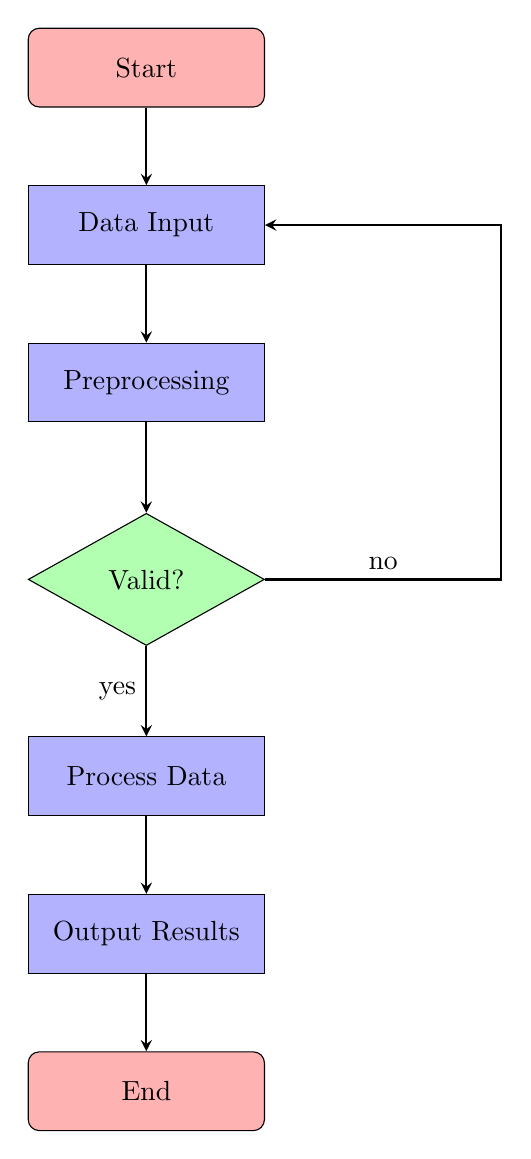
\begin{tikzpicture}[
        node distance=2cm,
        startstop/.style={rectangle, rounded corners, minimum width=3cm, minimum height=1cm, text centered, draw=black, fill=red!30},
        process/.style={rectangle, minimum width=3cm, minimum height=1cm, text centered, draw=black, fill=blue!30},
        decision/.style={diamond, minimum width=3cm, minimum height=1cm, text centered, draw=black, fill=green!30},
        arrow/.style={thick,->,>=stealth}
        ]
        
        \node (start) [startstop] {Start};
        \node (input) [process, below of=start] {Data Input};
        \node (preprocess) [process, below of=input] {Preprocessing};
        \node (decide) [decision, below of=preprocess, yshift=-0.5cm] {Valid?};
        \node (process) [process, below of=decide, yshift=-0.5cm] {Process Data};
        \node (output) [process, below of=process] {Output Results};
        \node (stop) [startstop, below of=output] {End};
        
        \draw [arrow] (start) -- (input);
        \draw [arrow] (input) -- (preprocess);
        \draw [arrow] (preprocess) -- (decide);
        \draw [arrow] (decide) -- node[anchor=east] {yes} (process);
        \draw [arrow] (decide.east) -- node[anchor=south] {no} ++(3,0) |- (input.east);
        \draw [arrow] (process) -- (output);
        \draw [arrow] (output) -- (stop);
        
    \end{tikzpicture}
    \caption{Data processing flowchart generated with AI assistance}
    \label{fig:flowchart}
\end{figure}

\subsection{Neural Network Architecture}

\textbf{Prompt:} "Generate TikZ code for a simple neural network with input, hidden, and output layers."

\begin{figure}[h]
    \centering
    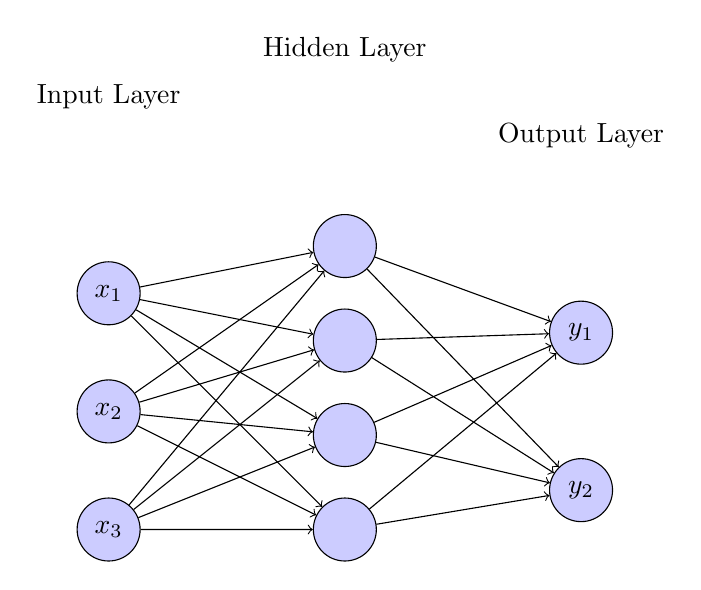
\begin{tikzpicture}[
        node distance=1.5cm,
        neuron/.style={circle, draw, minimum size=0.8cm, fill=blue!20},
        layer/.style={draw=none}
        ]
        
        % Input layer
        \foreach \i in {1,2,3}
            \node[neuron] (I\i) at (0,-\i*1.5) {$x_\i$};
        
        % Hidden layer
        \foreach \i in {1,2,3,4}
            \node[neuron] (H\i) at (3,-\i*1.2+0.3) {};
        
        % Output layer
        \foreach \i in {1,2}
            \node[neuron] (O\i) at (6,-\i*2) {$y_\i$};
        
        % Connections
        \foreach \i in {1,2,3}
            \foreach \j in {1,2,3,4}
                \draw[->] (I\i) -- (H\j);
        
        \foreach \i in {1,2,3,4}
            \foreach \j in {1,2}
                \draw[->] (H\i) -- (O\j);
        
        % Layer labels
        \node[above of=I1, yshift=1cm] {Input Layer};
        \node[above of=H1, yshift=1cm] {Hidden Layer};
        \node[above of=O1, yshift=1cm] {Output Layer};
        
    \end{tikzpicture}
    \caption{Neural network architecture diagram}
    \label{fig:neural_net}
\end{figure}

\subsection{Block Diagram}

\textbf{Prompt:} "Create a block diagram showing system components and data flow."

\begin{figure}[h]
    \centering
    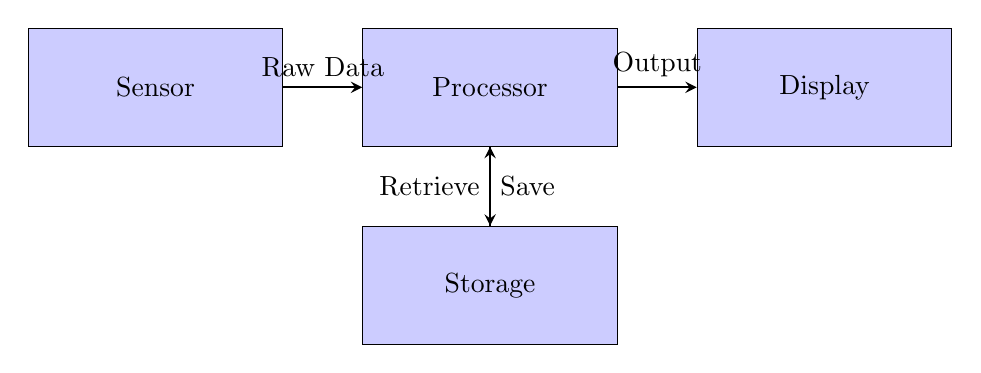
\begin{tikzpicture}[
        block/.style={rectangle, draw, fill=blue!20, text width=3cm, text centered, minimum height=1.5cm},
        arrow/.style={->, thick, >=stealth}
        ]
        
        \node[block] (sensor) {Sensor};
        \node[block, right=of sensor] (processor) {Processor};
        \node[block, right=of processor] (display) {Display};
        \node[block, below=of processor] (storage) {Storage};
        
        \draw[arrow] (sensor) -- node[above] {Raw Data} (processor);
        \draw[arrow] (processor) -- node[above] {Output} (display);
        \draw[arrow] (processor) -- node[right] {Save} (storage);
        \draw[arrow] (storage) -- node[left] {Retrieve} (processor);
        
    \end{tikzpicture}
    \caption{System block diagram}
    \label{fig:block_diagram}
\end{figure}

%==============================================================================
\section{Code Listings}

\subsection{Python Code Example}

\textbf{Prompt:} "Format this Python function with syntax highlighting using listings package."

\begin{lstlisting}[language=Python, caption={Python function for calculating factorial}, label=lst:factorial]
def factorial(n):
    """
    Calculate factorial of n recursively.
    
    Args:
        n (int): Non-negative integer
    
    Returns:
        int: Factorial of n
    """
    if n == 0 or n == 1:
        return 1
    else:
        return n * factorial(n - 1)

# Example usage
result = factorial(5)
print(f"5! = {result}")  # Output: 5! = 120
\end{lstlisting}

\subsection{R Code Example}

\textbf{Prompt:} "Show R code for linear regression with proper formatting."

\begin{lstlisting}[language=R, caption={Linear regression in R}, label=lst:regression]
# Load data
data <- read.csv("dataset.csv")

# Fit linear model
model <- lm(y ~ x1 + x2 + x3, data = data)

# View summary
summary(model)

# Plot residuals
plot(model$residuals)

# Predictions
predictions <- predict(model, newdata = test_data)
\end{lstlisting}

%==============================================================================
\section{Complex Structures}

\subsection{Multi-part Figures}

\textbf{Prompt:} "Create LaTeX code for 4 subfigures in a 2x2 layout."

\begin{figure}[h]
    \centering
    \begin{minipage}{0.48\textwidth}
        \centering
        \fbox{\parbox{0.9\textwidth}{\centering\vspace{1.5cm}Plot A\vspace{1.5cm}}}
        \caption*{(a) First plot}
    \end{minipage}
    \hfill
    \begin{minipage}{0.48\textwidth}
        \centering
        \fbox{\parbox{0.9\textwidth}{\centering\vspace{1.5cm}Plot B\vspace{1.5cm}}}
        \caption*{(b) Second plot}
    \end{minipage}
    
    \vspace{0.5cm}
    
    \begin{minipage}{0.48\textwidth}
        \centering
        \fbox{\parbox{0.9\textwidth}{\centering\vspace{1.5cm}Plot C\vspace{1.5cm}}}
        \caption*{(c) Third plot}
    \end{minipage}
    \hfill
    \begin{minipage}{0.48\textwidth}
        \centering
        \fbox{\parbox{0.9\textwidth}{\centering\vspace{1.5cm}Plot D\vspace{1.5cm}}}
        \caption*{(d) Fourth plot}
    \end{minipage}
    
    \caption{Comparison of four experimental results}
    \label{fig:multiplot}
\end{figure}

\subsection{Nested Lists}

\textbf{Prompt:} "Generate a nested list structure with three levels."

\begin{enumerate}
    \item \textbf{Data Collection Phase}
    \begin{itemize}
        \item Survey design
        \begin{itemize}
            \item Question formulation
            \item Pilot testing
            \item Refinement
        \end{itemize}
        \item Sample selection
        \item Data gathering
    \end{itemize}
    
    \item \textbf{Analysis Phase}
    \begin{itemize}
        \item Data cleaning
        \item Statistical analysis
        \begin{itemize}
            \item Descriptive statistics
            \item Inferential tests
            \item Correlation analysis
        \end{itemize}
        \item Interpretation
    \end{itemize}
    
    \item \textbf{Reporting Phase}
    \begin{itemize}
        \item Visualization creation
        \item Report writing
        \item Peer review
    \end{itemize}
\end{enumerate}

%==============================================================================
\section{Custom Environments}

\subsection{Theorem Environment}

\textbf{Prompt:} "Create a custom theorem environment with proper numbering."

\newtheorem{theorem}{Theorem}[section]
\newtheorem{lemma}[theorem]{Lemma}
\newtheorem{corollary}[theorem]{Corollary}

\begin{theorem}[Pythagorean Theorem]
In a right-angled triangle, the square of the hypotenuse equals the sum of squares of the other two sides.
\begin{equation}
    a^2 + b^2 = c^2
\end{equation}
\end{theorem}

\begin{lemma}
If $a$ and $b$ are positive real numbers, then $(a + b)^2 = a^2 + 2ab + b^2$.
\end{lemma}

\subsection{Definition Box}

\textbf{Prompt:} "Create a highlighted definition box."

\begin{center}
\fcolorbox{blue}{blue!10}{
\parbox{0.9\textwidth}{
\textbf{Definition (Machine Learning):}
Machine learning is a subset of artificial intelligence that enables systems to learn and improve from experience without being explicitly programmed.
}}
\end{center}

%==============================================================================
\section{Special Formatting}

\subsection{Highlighted Text}

\textbf{Prompt:} "Show different ways to highlight important text."

\begin{itemize}
    \item \textbf{Bold text} for emphasis
    \item \textit{Italic text} for definitions or foreign words
    \item \texttt{Monospace} for code or filenames
    \item \underline{Underlined} text (use sparingly)
    \item \textcolor{red}{Colored text} for warnings
    \item \textcolor{blue}{\textbf{Combined formatting}} for maximum emphasis
\end{itemize}

\subsection{Custom Commands Created by AI}

\textbf{Prompt:} "Create custom LaTeX commands for frequently used terms."

% Custom commands
\newcommand{\suza}{State University of Zanzibar (SUZA)}
\newcommand{\ml}{machine learning}
\newcommand{\ai}{artificial intelligence}

Example usage:
The \suza{} is conducting research on \ml{} applications in \ai{}.

%==============================================================================
\section{Lessons Learned}

\subsection{AI Strengths}
\begin{itemize}
    \item Rapid generation of boilerplate code
    \item Correct syntax for complex structures
    \item Creative solutions to formatting problems
    \item Quick debugging of error messages
    \item Consistent formatting across elements
\end{itemize}

\subsection{AI Limitations}
\begin{itemize}
    \item May produce outdated package syntax
    \item Cannot verify factual accuracy
    \item Sometimes overcomplicates simple tasks
    \item Requires human review and testing
    \item May not follow specific style guidelines
\end{itemize}

\subsection{Best Practices}
\begin{enumerate}
    \item Always test generated code before use
    \item Verify package compatibility
    \item Understand the code, don't just copy-paste
    \item Iterate and refine prompts for better results
    \item Document AI assistance in your workflow
    \item Maintain academic integrity
\end{enumerate}

%==============================================================================
\section{Conclusion}

This document has demonstrated various types of LaTeX code that can be generated with AI assistance. While AI is a powerful tool for accelerating LaTeX development, it should be used thoughtfully and always verified.

\textbf{Key Takeaway:} AI is an excellent assistant but not a replacement for understanding LaTeX fundamentals and critical thinking.

\vspace{2em}

\begin{center}
\fbox{\parbox{0.8\textwidth}{\centering
\textbf{Remember:}\\[0.5em]
\textit{"AI-assisted does not mean AI-generated.\\
You are still the author of your work."}
}}
\end{center}

%==============================================================================
\appendix

\section{Prompt Engineering Tips}

\begin{enumerate}
    \item \textbf{Be Specific}: Include document class, packages, and desired output
    \item \textbf{Provide Context}: Mention your field and intended use
    \item \textbf{Request Explanations}: Ask AI to explain what the code does
    \item \textbf{Iterate}: Refine based on initial output
    \item \textbf{Test Thoroughly}: Compile and verify all generated code
\end{enumerate}

\section{Verification Checklist}

Before using AI-generated LaTeX code:
\begin{itemize}
    \item[$\square$] Code compiles without errors
    \item[$\square$] Output matches intended design
    \item[$\square$] All packages are loaded correctly
    \item[$\square$] Cross-references work properly
    \item[$\square$] Numbering is consistent
    \item[$\square$] Code is properly commented
    \item[$\square$] Style matches document requirements
\end{itemize}

%==============================================================================
\end{document}